\documentclass[a4paper]{article}

\usepackage[english]{babel}
\usepackage[utf8x]{inputenc}
\usepackage{amsmath}
\usepackage{graphicx}
\usepackage[colorinlistoftodos]{todonotes}
\usepackage{wasysym}
\usepackage{hyperref}

\title{Analysis of a Contemporary Data : Upvotes \& Downvotes}
\author{Buse Gul Atli \\ buse.atli@aalto.fi}

\begin{document}
\maketitle

\begin{abstract}
Social media has a great source for analyzing community opinions about specific topic. However, it is hard to find a good data for general threads to estimate what is the most frequent and broad topic worldwide. This report aims to find the most popular topics and the frequency of comments by investigating data collected from Reddit which a popular site with rich content. Tableau tool and Python 2.7 are used for understanding and analyzing the data.  
\end{abstract}

\section{Introduction}
Social networks is currently gaining an increased amount of popularity. Content submitting, voting, commenting have become our daily jobs. In a day, millions of threads and subreddits are created and voted. When we get up in the morning, most of us check social media such as Facebook Twitter, 9gag, Reddit etc and like some posts, comment on threads. For instance, Reddit achieved 82.54 billion page views, 73.15 million submissions, 725.85 million comments and 6.89 billions upvotes just in 2015\cite{intro}. This research was done using Stanford Reddit dataset collections to find an answer the following questions:\
What could be a candidate the highly discussed topics with pictures in social media?\
Can we correlate other popular media items to the frequency of posts?\
Do people comment on the posts they like/ dislike?\
Is the voting community important to get higher like?\
\subsection{Design Methods}
The report followed Munzner's Model of visualization design and validation techniques \cite{munzner} Audience is obviously anyone who has an interest on social media, especially Reddit. Therefore, the tasks are simple identifications and comparisons. Downloaded dataset type is table with multiple items and attributes. Since the dataset is massive, answering to the questions in Introduction section is quite hard. On the other hand, visual encoding of this table can give a better understanding for the goals. For this reasons, charts are based on scatterplots and preattentive features such as size and color to have the effectiveness of visual variables and to get the answers. Furthermore, Gantt chart is used to visualize the posting times to quickly infer the time starts for increase in topic popularity. While creating the visual graphs, Tufte's principles about showing the data and avoiding distortions are also considered.

\section{Data Description and Approach}
The related dataset is downloaded from Stanford Large Network Dataset Collection and it includes 132,308 Reddit submissions from 2008 to 2013. Reddit.com is a social media site where users can create content or comment and evaluate these. The negative and positive feedback called upvotes and downvotes to a particular content gives an overal score to promote the content. If a content obtains higher rate, it will be visible in top pages. Content can be completely public or posted to subreddits. Subreddits are large communties with a specific theme, so a content can get less view but more rate when it is submitted to these pages. All submissions are an image uploaded with a particular title to a specific subreddit in a known date. Subreddits are subtopics in the Reddit website so that communities can move from one of them to another and see a submission with a title. Moreover, same contents are resubmitted multiple times with multiple titles to multiple communities \cite{dataset}. Hence, a same content can get different scores in terms of upvotes, downvotes and comment. The dataset also consists of the author and the UNIX time(epoch) for each title.
Collected statistical data has been refined to eliminate adult content or title by using simple language processing algorithms by using Python. Although this could affect the overall results, there has been little change in the distributions with this excluded information. The statistics used for this report about the dataset can be seen in Table~\ref{table:dataset}. Tableu visualization tool is used to create desired graphs because of the aesthetic concerns and painless creation of desired charts.   
\begin{table}
\centering
\begin{tabular}{l|r}
Info & Statistics \\\hline
Total number of images  & 132,307 \\
Total number of communities(subreddits) & 867 \\
Total number of comments &5,168,289 \\
Total number of ratings & 249,168,951
\end{tabular}
\caption{\label{table:dataset}Statistics for the Reddit Data}
\end{table}

\section{Analysis of the Data}
Firstly, Reddit data was grouped in subreddits and the total number of comments and votes are obtained. In the Figure~\ref{fig:topics}, each bubble represents the subreddit. The size of the bubble describes the number of votes for specific content. Furthermore, the saturation represents the number of votes for each subreddit. As seen in the figure:\ref{fig:topics}, there is high correlation between total votes and comments. It can be inferred that people most likely tends to comment on a submission they vote. 
Secondly, the time of the each post with respect to the subreddit they are in is analyzed.(Figure:\ref{fig:freq}) Time dimension is shown as UNIX time. When they are converted to human readable from, there is quite less activity before 2010(1280M). Actually, Reddit has become widely known since 2010, so the data is completely consistent with this trivia. Moreover, the most frequent subreddits are the most voted and commented ones when we compared to this figure to figure~\ref{fig:topics}, as expected. There is a special subreddit called Breaking Bad which is a famous TV show. The first submission was around 2010 when this show was airing 3th season and from this season the viewers of this series has increased drastically. This graph can relate many social information like this example. 
Finally, an upvote\& downvote\& scoring for selected subreddits chart is created to scrutinize the possible relationships.(Figure~\ref{fig:votes}) We can say that even though total vote for funny theme is the highest, it contains many downvotes too. The same phenomenon occurs for "pics", "WTF" and "gifs" subreddits. Another great information from this chart is the name of topics. For example, the content of the submissions for "Fun" and "funny" is similar; however, the rating values are so different. wWhen we compare the findings for the "aww"\& "Awww", "Games"\& "gaming", "gif"\& "gifs" and "WTF"\& "wtfart", the same contrast can be spotted. This brings the importance of the idea about selecting more crowded community or posting a thread to a community with comparable taste. If a user submits to populous area of reddit, he has the possibility to get higher vote. On the contrary, there will be more posts so his topic can became less popular. 
\begin{figure}
\centering
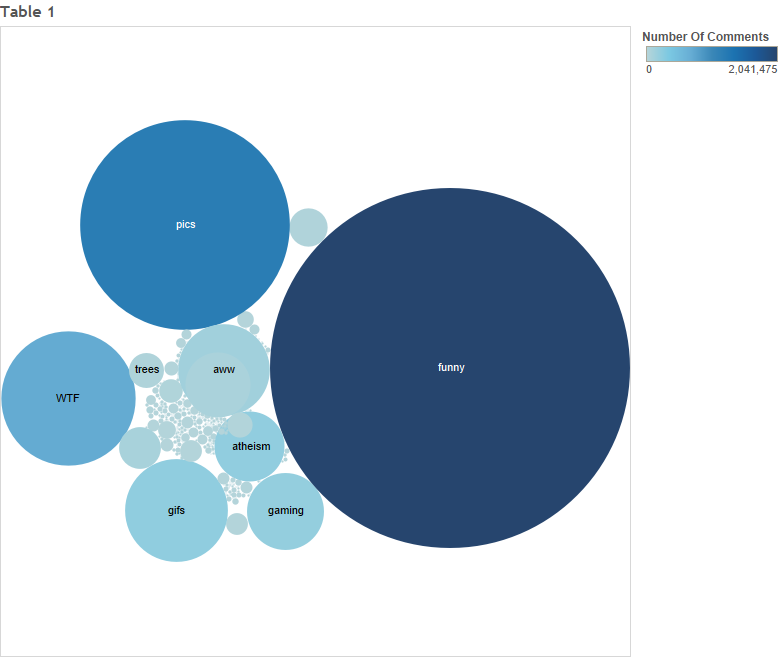
\includegraphics[width=0.8\textwidth]{topicss.png}
\centering
\caption{\label{fig:topics}The Distribution of Subreddits}
\end{figure}
\begin{figure}
\centering
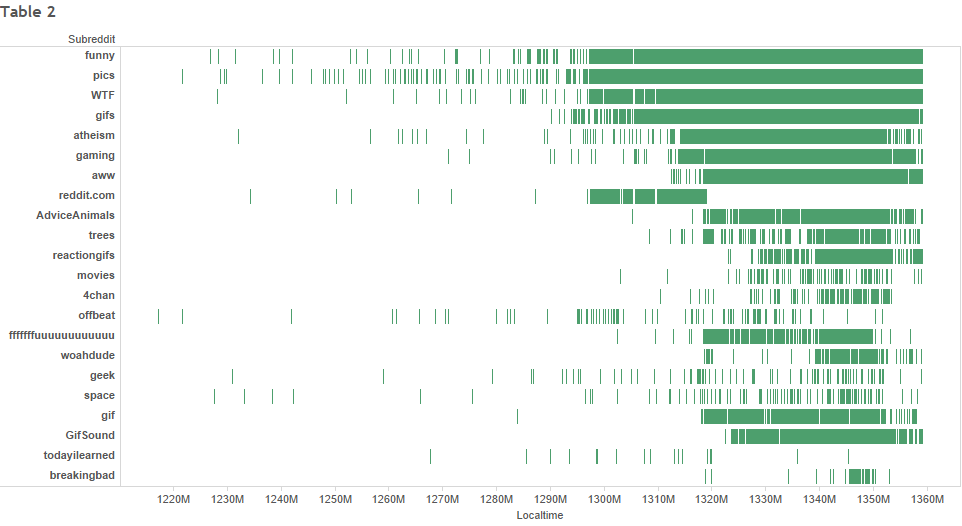
\includegraphics[width=1\textwidth]{times.png}
\centering
\caption{\label{fig:freq}The Commenting Frequency of Subreddits}
\end{figure}
\begin{figure}
\centering
\fbox{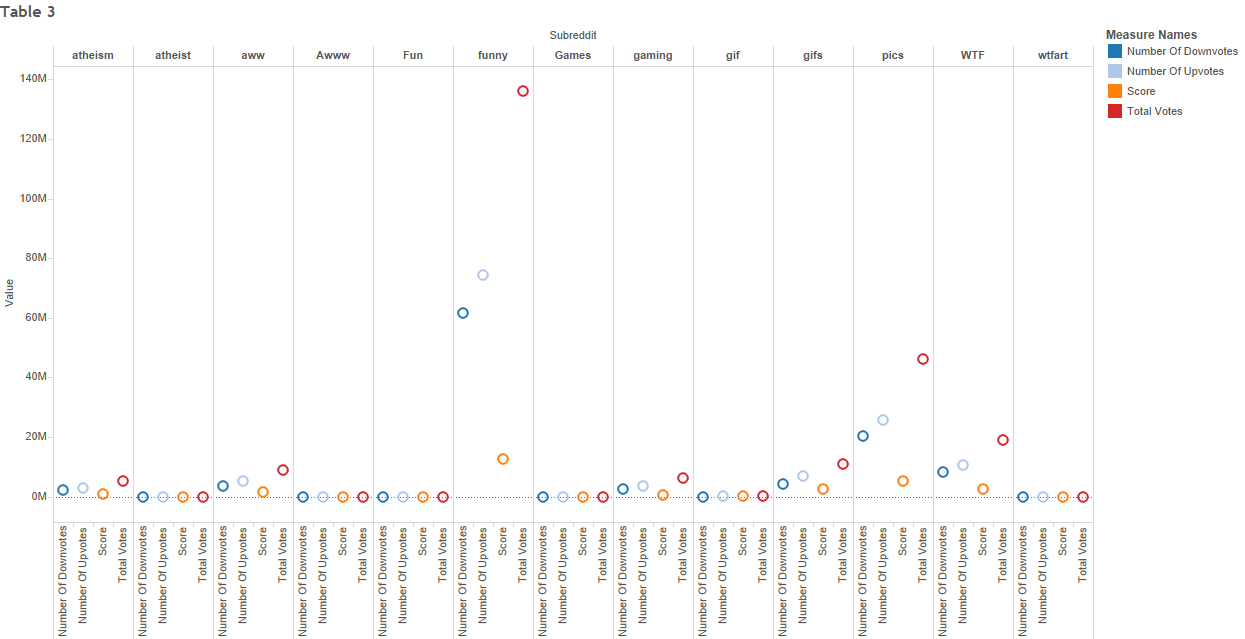
\includegraphics[width=1\textwidth]{votings.png}}
\centering
\caption{\label{fig:votes}Upvote \& DownVote for Subreddits}
\end{figure}

\section{Conclusion}
In this report, the aim was to find the widely discussed topics in social media, finding correlation between voting and commenting and to relate the statistics to a social topic. Reddit Data collected by Stanford University was analyzed and the obtained results gave promising implications. It was not surprising to see the "funny" themed topics have the most reactions and the graphs proved there is an analogy between commenting and voting rate. The subreddit header is also important to get more attention from different communities. In addition to the answered questions, the charts also asserts that a popular subreddit can have both high upvotes and downvotes so the overall score may be lower than expected. 
In conclusion, with the help of visualization about huge dataset of social media to have a general idea about what and when society is thinking most and how they react to other's thoughts. This is the most valuable information for companies to take actions in our internet-driven world. 
\begin{thebibliography}{1}
\bibitem{dataset} 
Lakkaraju H., McAuley J., Leskovec J., 2013. \textit{What's In a Name? Understanding the Interplay Between Titles, Content, and Communities In Social Media}, ICWSM.
\bibitem{munzner}
Micallef L., and Munzner T., 14-03-2016. \textit{Information Visualization Lecture 7: Visualization Analysis \& Design},Lecture
\bibitem{intro} 
\textit{Reddit.com Traffic Statistics}
\url{https://www.similarweb.com/website/reddit.com} 
. Similar Web
Retrieved 2016-12-04
\end{thebibliography}

\end{document}